%%% 1 Introduction/ %%%
\chapter{Introduction}\label{ch:intro}
%WHAT - what the reader needs to know to understand the presented 
%work, explain the background of research
%Society, Honesty difficult to predict, spy problem.
%only way - to constantly get feedback about the current behavior
%prisoner's dilemma an expermient that suggests, people act honestly if there is 
% long term benefit 
%i.e., if a user might have to interact again with the same person for some
%reason, then they are more likely to behave honestly. 
We rely heavily on the internet today, from using emails to communicate with
one another, searching for an online source of news or media files to shopping
for everyday things. One can say that the internet has become an inseparable
part of our society. Statistics~\cite{InternetWorldStat} suggest that there are
approximately 4 billion internet users worldwide and this number is only
increasing with each passing day. Internet live stats~\cite{InternetLiveStat}
is an online service that provides live statistics on various online activities
such as blog posts, social media usage, internet traffic and emails sent. Given
the global reach of the internet and diversity of users, one can reasonably
assume that not all online interactions happen between known entities. The
online identities that everyone uses to interact with one another provide no
way to confirm the real-world identity or the attitude of the person behind. To
determine the trustworthiness of an entity is a difficult task even in the real
world. If Alice needs to interact with Bob, she has no way of measuring the
trustworthiness of Bob with 100\% certainty. She could get a reference from
others in the society, i.e., by referring to Bob's reputation. If Bob has a
good standing among members of the community due to good records or other
objective measures, there is a high probability that Alice's interaction with
Bob will result in a good outcome, i.e., Alice's perception of Bob being good
will turn out to be true. However, this does not provide any guarantee of Bob's
behavior. Bob could be a malicious actor who was waiting for the right moment
to deal severe damage. There is no way of guaranteeing that the behavior of an
entity will always be an honest one. Honesty can be seen as an attribute at a
given time. Alice may trust Bob today but not tomorrow because he may have
taken a damaging action. Depending on the damage caused by his action, the
level of trustworthiness also gets affected. As such, anyone can be seen as
honest until they deal damage and are known as a malicious actor. That is when
they lose their reputation, and other members are less likely to trust them. \par
This notion of trust and reputation, when used in online interactions, can help
to predict the outcome of online transactions. Any online platform where users
communicate with each other for different purposes (e.g., digital transaction,
news or file sharing) can be termed as online interaction system. Depending on
the nature of the interaction, the failing outcome can have a significant
impact on interacting entities. For instance, the failure of an interaction
that involves buying a house is not the same as failing to receive a
high-quality music file. To prevent severe damage that might result from a
failed transaction, trust frameworks and reputation models of the interaction
system play a crucial role. They attempt to avoid harm by giving enough
information about the interacting entities to be able to predict the outcome. A
reputation system collects information about the interacting entities by
continually updating the state based on feedback. The risk of failure or
probability of success when interacting with an entity relies on the
information provided by the underlying reputation system. This information is
usually presented in the form of trust scores assigned to each online identity.
Before engaging in an online transaction, the entities need to select the
online identity of the user with whom they intend to interact. The interaction
can then take place whose outcome is observed and stored by the reputation
system to update the current trust value further. Examples of reputation
systems in use by current online interaction platform are
eBay~\footnote{https://www.ebay.com/}, which is an e-commerce platform,
StackExchange~\footnote{https://stackexchange.com/}, which is a Q\&A platform,
and Reddit~\footnote{https://www.reddit.com/}, which is a content rating and
discussion platform. The trust score of users is based on their feedback,
positive/negative ratings, upvotes/downvotes from the participants with an
equal privilege to interact with the system. The final score aggregated via
these measures can either raise or lower the reputation of the user and limit
their interaction ability.  \par
\begin{figure}[H]
	\begin{center}
		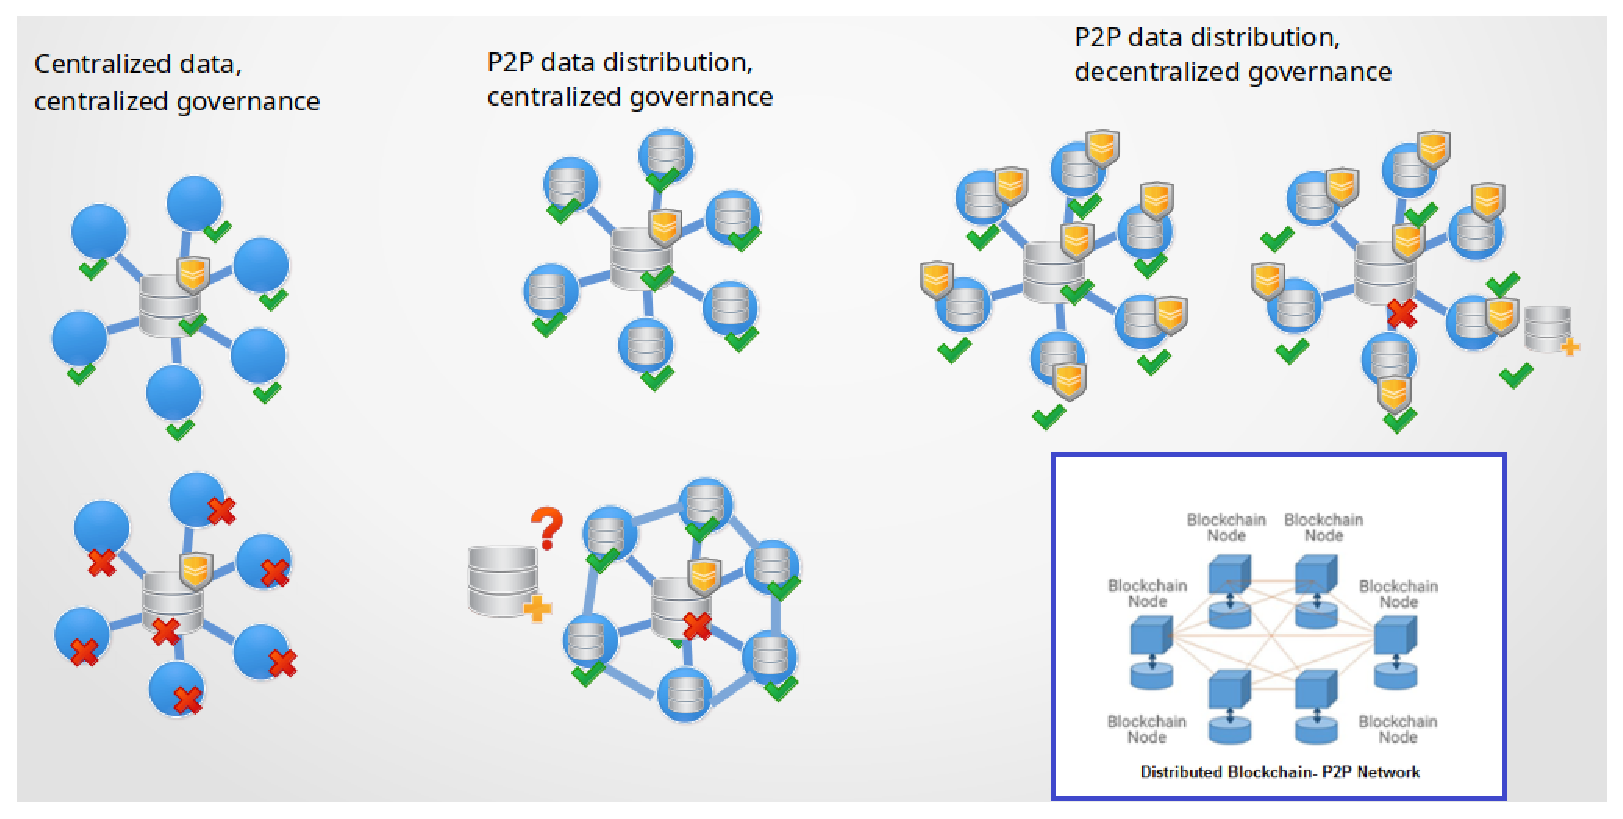
\includegraphics[width=1.0\textwidth]{Images/WhyBlockchain.eps}
		\caption{Centralized vs. decentralized network}
		\label{fig:WhyBlockchain}
	\end{center}
\end{figure}
\vspace{-8mm}
A general trust framework and a good reputation model to specify the rules of
interaction between online identities and the extraction of useful information
from them is, therefore, essential to maintaining the security of an online
interaction system. Equally significant is to protect the integrity of this
information such that they are reliable, untampered (no deliberate alteration
of data) and always available. Most of the online interaction systems make use
of a client-server architecture to serve and govern the data usage. As such,
the system is centralized and prone to both external attacks and internal
modifications. If the server nodes fails, then the whole network fails since
none of the clients can access the data anymore. An alternative architecture
that is primarily utilized by file sharing systems is a ~\ac{P2P} network, and
reputation-based trust management system for them exists as
well~\cite{selcuk2004reputation}. In a ~\ac{P2P} network, all nodes (peers) can
act as both client and server, i.e., a peer can both request and serve data.
Thus, if one node fails, clients can still request data from other nodes in the
network. Earlier P2P file-sharing services such as
Napster~\cite{stern2000napster} offered P2P data distribution such that clients
could request data from any nodes connected to its network. However, the
drawback of this system was that it kept a central server to index the location
of files. This form of centralized data governance acted as a single point of
failure, and the shutdown of its service was possible. Other P2P file-sharing
services that followed employed a decentralized and distributed indexing method
to overcome this vulnerability. Example include
BitTorrent~\cite{cohen2003incentives,cohen2008bittorrent}, which allowed the
participating nodes to track the location of a file (to discover peer) without
the use of a central server. Blockchain technology~\cite{pilkington201611}
makes use of a P2P network although its main design goal was not that of a
file-sharing service but instead started as a way to store and distribute data
over the network in an immutable fashion. It allows the nodes to store blocks
of data chained together in a cryptographically secure method such that the
modification of stored data is computationally infeasible. These models can be
seen in Figure~\ref{fig:WhyBlockchain} in Section~\ref{ch:intro}.  \par
\begin{figure}[H]
	\begin{center}
		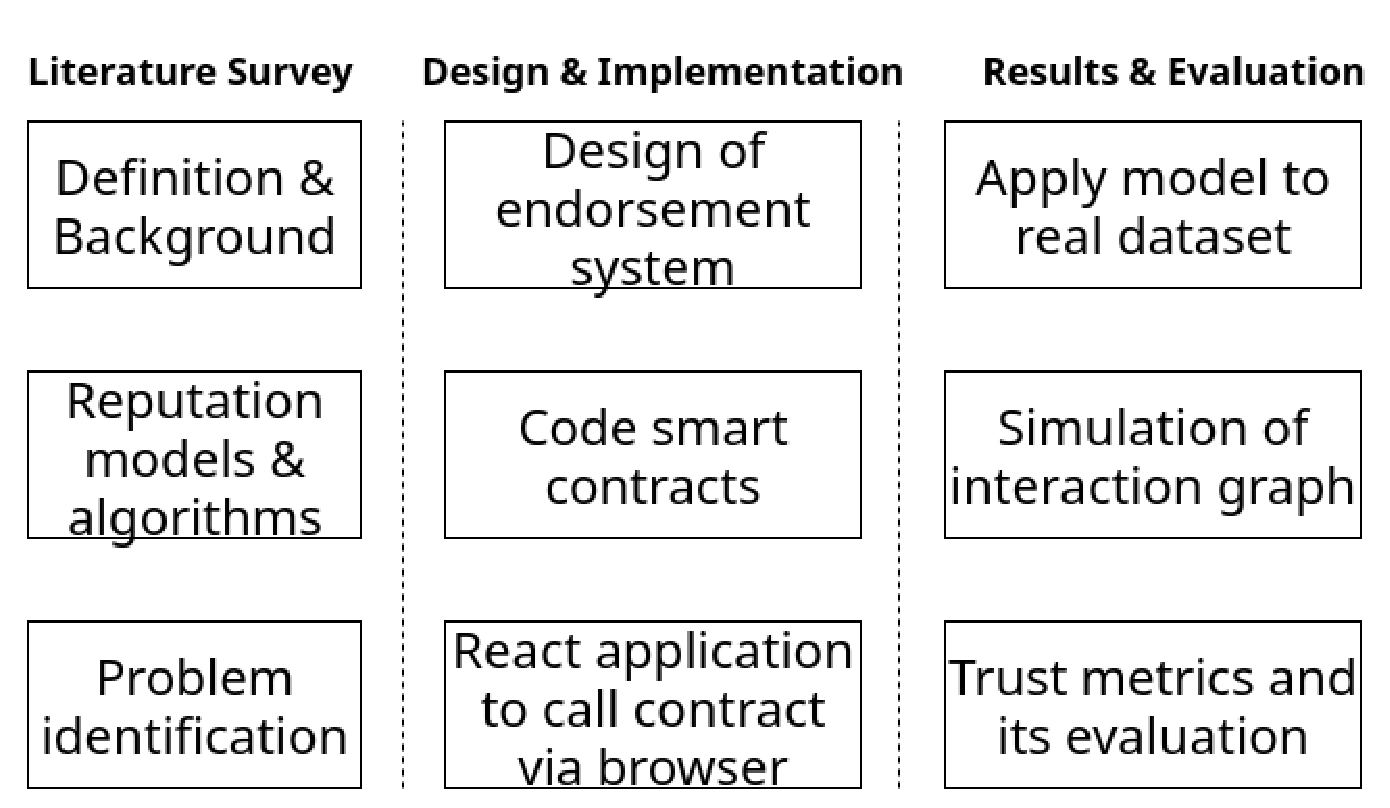
\includegraphics[width=0.9\textwidth]{Images/workflow.eps}
		\caption{Phases of the project.}
		\label{fig:thesisSteps}
	\end{center}
\end{figure}
\vspace{-8mm}
This master’s thesis project, therefore, proposes the use of blockchain
technology and smart contracts to model a trust framework and implement a
reputation system. The initial step of the project was the identification of
relevant concepts by performing a literature survey on existing reputation
models, properties of graph-based algorithms and its relevance to the project.
The survey motivated the design of a solution, wherein the proposed model,
participating entities can endorse each other. Based on assumptions about
different possibilities of endorsement behavior that may occur, trust metrics
were defined in a way that honest participation would be encouraged. The
definition of honest and malicious participation from the perspective of an
endorsement network is discussed in Section~\ref{ch:method}. A method to
collect and quantify this endorsement information to assign a trust score to
each entity is presented. To assess the working of the proposed model, it is
applied to an existing real dataset. Computation of trust scores for each
participant based on the defined trust metrics is presented. The simulated
graph and computed trust scores do support the defined metrics. A discussion of
relevant threat models on reputation systems and how the proposed model
addresses them is presented. Different phases of this master's thesis project
are given by Figure~\ref{fig:thesisSteps}.\par
The major contribution of this master's thesis project is:
\begin{itemize}
	\item Design of an endorsement model where entities can endorse information
		about each other and a method to aggregate this information such that a
		global value can be assigned to individual entities to infer their
		trustworthiness.
	\item Deployment of the endorsement system on blockchain network that
		updates and computes the trust scores of entities by executing the
		smart contract code based on users' interaction ensuring reliable and
		verifiable information. 
	\item Evaluation of the endorsement model by applying it to an existing
		data set and discussion of relevant threat models.
\end{itemize}

%and therefore can be stated as a soft
%security mechanism. Rasmusson, Lars and Jansson,
%Sverker~\cite{rasmusson1996simulated} first used this term to describe the idea
%of identifying malicious users and preventing harm to other users in the
%context of secure open electronic commerce. Here, it is up to the individuals
%rather than the software to maintain security.

%\begin{wrapfigure}{l}{0.6\textwidth}
%	\begin{center}
%		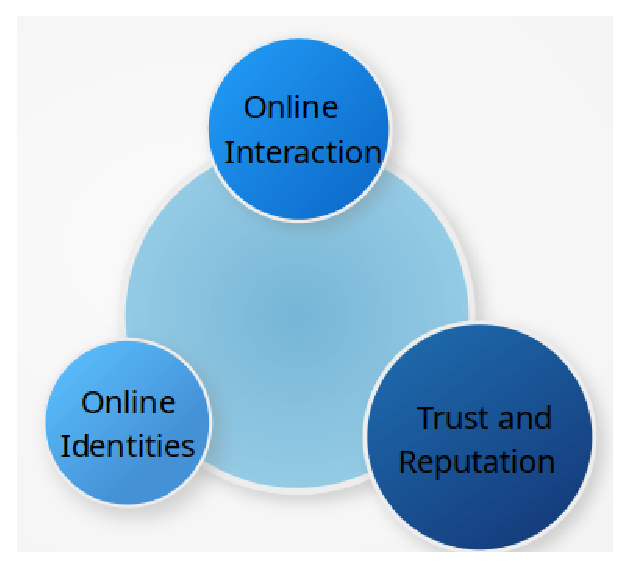
\includegraphics[width=0.5\textwidth]{Images/Introduction.eps}
%		\caption{Online identities and their interaction}}
%		\label{fig:introduction}
%	\end{center}
%\end{wrapfigure}
 
\section{Motivation}
%WHY: why is it interesting to study reputation system/trust 
% why blockchain based solution is relevant/interesting
Consider a simple scenario where Alice wants to buy a pair of headphones for
which she browses a ``buy/sell'' platform. When she finds a relevant product on
the platform published by Bob, an unknown entity to Alice, the success or
failure of the transaction depends on two factors that may or may not be
transparent.
\paragraph{Reputation of Bob:} Reputation of Bob can be inferred from his
history of transactions, ratings provided by previous buyers that have dealt
with him, the reputation system of the platform in use and the integrity of all
these relevant data.  
\paragraph{Reputation of the platform:} This factor can also be inferred
similarly based on the history of services the platform has been able to
provide or a general perception in the community. Here, the platform in use
acts as the trusted third party that Alice must trust to present correctly
computed, untampered data about Bob or the ad posted by him. The entity
claiming to be Bob could be Eve, who found a way to bypass the security of the
platform in use to inflate her reputation. Eve could delete the ad and
associated account when the payment is complete, or she could gather details
about Alice to misuse it later. Any malformed decision on the trustworthiness
of an entity could be expensive and deal severe damage to the user. \par
Statistics suggest that online shopping is the most adapted online
activity~\cite{experian}. Reports by Experia~\cite{experian} and
Javelin~\cite{javelin} indicate that E-commerce fraud has increased by 30\% in
2017 over 2016 while identity fraud victims have risen by 8\% in 2017 (16.7
million U.S. victims). A recent report of the data breach~\cite{macy} on an
online shopping website, Macy~\footnote{https://www.macys.com/}, exposed its
users' information such as their name, credit card number, expiry date. While
there are several security reasons that have led to attack at such scale, one
reason is the client-server architecture where everything is stored on
centralized server and data flows in and out from the same source. On the other
hand, distributing information over a decentralized network would require
simultaneous attack to achieve the same effect, thereby increasing the
difficulty level of attack. Similarly, Reputation models can help in measuring
the reliability of interacting entities so that users can make an informed
decision before participating in any transaction. Thus, a reputation system
should be secure, robust, always available and aim for higher accuracy. The use
of right reputation algorithms with blockchain technology could help to ensure
the trustworthiness of online entities with the correctness of data and a high
degree of accuracy.  
 
%Additionally, reports on fake news
%\footnote{\url{https://journalistsresource.org/studies/society/internet/fake-news-conspiracy-theories-journalism-research}}$^{,}$\footnote{\url{https://www.prnewswire.com/news-releases/84-percent-of-businesses-could-reduce-fraud-risk-if-certain-about-customers-identity-300587192.html}}
%that leads to spread of misinformation from malicious users or portals, attack
%on an existing system continues.
%while Facebook has admitted to the compromise of
%2.2 billion of its user's data
%\footnote{\url{https://thenextweb.com/facebook/2018/04/05/zuckerberg-facebooks-2-billion-users-assume-data-compromised/}}.
%\footnote{\url{https://thehackernews.com/2018/04/facebook-data-privacy.html}}.
%generalize a trust framework is, therefore, a riveting problem. Graph theory
%and network flow algorithms have been researched in both centralized and
%decentralized environment before. This thesis proposes a blockchain based
%solution to record users behavior and compute a trust score for each of them. 
\section{Purpose and research questions} \label{ResearchQuestions}
%Goal of thesis
%Research questions and approach that will be taken to answer 
%them in brief.
The primary goal of this master's thesis project is to use blockchain
technology and smart contracts to model an interaction system where entities
can endorse each other. It aims to specify the rules of interaction and provide
a method to aggregate these interactions to generate a trust score for the
interacting entities. The research questions that this project aims to address
are: 
%The primary goal of this master's thesis project is to use blockchain technology
%and smart contracts to simulate an endorsement network where entities can
%endorse each other based on physical or digital acquaintance. The endorsement
%will be quantified to infer reputation score which in turn can yield a value
%that can represent the impact the agent has made on the network.  The nodes and
%their relationship will be studied to analyze honest or malicious
%participation.  Generalization of this endorsement network to serve other use
%cases shall be discussed as well. \par
\begin{itemize}
%		\item How can graph theories and relevant reputation algorithms be used
%			to model the interaction between entities and identify honest and
%			malicious nodes in the network? \label{question1}
		\item What are the requirements for storing trust values and linking
			them to associated identities stored on or off a blockchain
			network? How can a blockchain application be built to define a
			general trust framework and how would the overall system
			architecture look like?\label{question2} 
		\item How can the proposed model help to infer the trustworthiness of
			interacting entities while preserving the anonymity of its users? 
\end{itemize}
\section{Scope} 
%Identify goal, objective, timeplan, deliverables, 
%what the project is supposed to do and the work required to meet 
%the objective
This master's thesis project attempts to answer the research questions
mentioned in Section~\ref{ResearchQuestions}.  
%\paragraph{Research Question 1}
%To answer research question 1, a literature survey is performed on various
%reputation algorithms and trust models. This survey follows with the discussion
%on various analysis metrics and threat models that eventually leads to graph
%simulation of an endorsement network.

\paragraph{Research Question 1 } 
An interpretation of connections between nodes and quantification of a score
that can represent trustworthiness of an entity is presented. Overall system
design and architecture to implement the application on blockchain network is
presented along with a comparative analysis of an on-chain vs. off-chain
storage.

\paragraph{Research Question 2} 
The study of threat models relevant to trust and reputation systems is
presented along with a discussion on how the proposed system addresses them. 
%For research question\ref{question2}, interpretation and quantification of reputation
%scores and trust metrics will be manifested. Comparative analysis of on chain
%and off-chain storage requirements will be studied resulting in an overall
%design of endorsement system architecture. \\
%\textbf{Research Question 3}
%The endorsement network will be analysed against various network metrics to show resilience to threat models. Discussion on other use cases and how the endorsement model can be used on top of other system will be presented. 
%

%For research question\ref{question3}, relevant use cases will be presented, and the
%network will be tested on with various predefined cases and attack models to
%see how well it behaves in a dynamic environment. \\

\section{Structure of Report}
This report is structured as follows. Chapter~\ref{ch:background} provides a
background overview of relevant concepts necessary to understand the following
sections. Chapter~\ref{ch:litrev} presents a literature survey on the existing
algorithms and their implementations. In Chapter~\ref{ch:method}, system
requirements and the approach taken for the model design are shown. It presents
the overall design and architecture of the proposed system.
Chapter~\ref{ch:results} presents the results and evaluation of the system
requirements. In Chapter~\ref{ch:discussion}, the discussion and analysis of
the overall project along with the limitations of the proposed system are
presented. Finally, conclusion and future works are presented in
Chapter~\ref{ch:conclusion}.
